\documentclass[11pt]{article}

%=============================================================================
% Everything between the '=' is the preamble.
%
% This is where document metadata is declared, as well as where we pull in any
% packages we might need for our document.
%
% Let's start with metadata
\title{Example Lab Report}
\author{Ross B.}
\date{\today}

% Here are our packages
\usepackage{amsmath}    % More math environments (like align) and capabilities
\usepackage{amssymb}    % More mathematical symbols
\usepackage{amsfonts}   % More fonts for math

\usepackage{graphicx}   % Standard package for including figures
%=============================================================================

\begin{document}

% This command compiles our metadata in the preamble into a nice title/heading
% for our document
\maketitle

\section{Introduction}
% Use `` for right-tailed quotation marks, and '' for left-tailed.
We're pretending to write a ``lab report'' to help us learn the basics of
\LaTeX. % This command renders a fancy LaTeX!
Let's use Arthur H. Compton's work on inelastic photon scattering as an 
example.

Putting a blank line between blocks of text in the .tex file result in a new
paragraph in the document.

\subsection{History}
\label{sec:nobel}
A.H. Compton was a physicist who, in 1927, shared the Nobel prize in physics 
for the ``discovery'' of inelastic photon scattering (a.k.a. Compton
scattering).

% Note: you can suppress the numbering of sections/subsections/subsubsections
% by adding an * before the brackets, like so:
\subsubsection*{Childhood}
A.H. Compton was born in Wooster, Ohio in the 1890's... 
\subsubsection*{WWII}
He was also a bigshot in the Manhattan Project


\section{Theory}
\label{sec:theory}

\LaTeX has become the standard markup for mathematical typesetting. 
Even if you don't use \LaTeX to make documents, chances are you will eventually
run into \LaTeX's syntax for math sooner or later if you're in a STEM field.
For example, the popular python plotting package matplotlib supports \LaTeX
syntax rendering for titles, axes labels, and other text.

In \LaTeX, mathematical expressions can be expressed within text by putting
the math expression betwee dollar signs.
For instance, we can express the equation for the Gaussian (or normal) 
distribution like so:
$f(x) = \frac{1}{\sqrt{2\pi\sigma}} e^{\frac{(x - \mu)^2}{2\pi\sigma^2}}$

Sometimes you want equations on their own lines, along with a reference number.
This is possible with the equation environment:

\begin{equation}
  E_{\gamma_{s}} = \frac{E_0}{1 + \frac{E_0}{mc^2}(1 - \cos{\theta})}
  \label{eqn:compton}
\end{equation}

With a little practice, writing mathematical expressions in \LaTeX syntax
becomes a breeze.
Also: google is your friend! There are tons and tons of different symbols and
built-in expressions: way more than you could ever hope to remember.

It's important to remember that this document has only the absolute basics
when it comes to expressing math.
There is a ton more out there, much of which is provided in \LaTeX 
packages from the American Mathematical Society (see preamble).
For example, what if we want several related equations to be aligned on the
page, with some text in between the equations?
% NOTE: you can italicize words using \emph{} or \textit{}, and make words
% bolded using the \textbf{} command.
We can do this with the \textbf{align} environment, which is available in the
\emph{amsmath} package.

% The WRONG way to reference your equations/figures/tables:
  % The above equation can be written in a simpler form as
% The RIGHT way to do it, using \label and \ref:
Equation \ref{eqn:compton} can be written in a simpler form as:

\begin{align}
  &\cos{\theta} = \frac{1}{A_{0}} - \frac{1}{A_{d}}
  \intertext{where}
  &A_{0} = \frac{E_{0}}{mc^{2}}
  \intertext{and}
  &A_{d} = \frac{E_{\gamma_{s}}}{mc^{2}}
\end{align}

\section{Methods}

% You can \label almost everything in latex so that you can reference those
% things later. Here, we reference a section that we had labeled above:
As mentioned in section \ref{sec:nobel}, the goal of this lab report is to win
a Nobel prize.

\subsection{Theoretical Preparation}

You can make numbered lists using the \emph{enumerate} environment:

\begin{enumerate}
  \item Write down the equations for relativistic conservation of energy and
        momentum.
  \item Do a little algebraic manipulation...
  \item Book a flight to Stockholm.
\end{enumerate}

\subsection{Experimental Preparation}

And bulleted lists with the \emph{itemize} environment:
List of required equipment to verify the theory in section \ref{sec:theory}

\begin{itemize}
  \item X-ray generator
  \item Scattering materials
        \begin{enumerate}
          \item wood
          \item lead
        \end{enumerate}
  \item Spectrometer
\end{itemize}

\section{Results}
Compton's pals Oskar Klein and Yoshio Nishina took Compton's work a step
further, and expanded on his theory.
In the results section, we'll show their results by including a plot showing
the theory, and give proper credit by citing their work.

We start with a figure generated from their theory.
We found a Klein-Nishina plot with a google-image search, and downloaded the
.png into this directory.
We can now include this image in our report using the \emph{includegraphics}
command from the \emph{graphicx} package (see the preamble).
The results of Klein-Nishina's theory are shown in figure \ref{fig:kn_plot}.

% A 'floating' figure environment. See the "bodies.pdf" slides in the ../bodies
% directory for more details.
\begin{figure}[htbp]
  % We want the figure in the center of the page, so we use the center
  % environment
  \begin{center}
  % Scale our image relative to the original photo size:
%  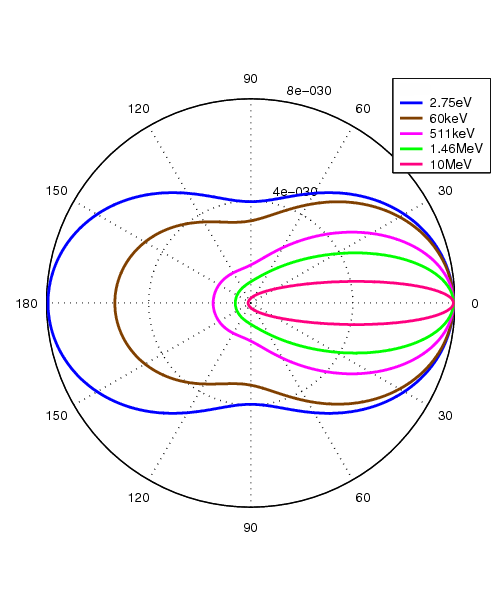
\includegraphics[scale=0.3]{Klein-Nishina_distribution.png}
  % Scale our image relative to the size of the page
  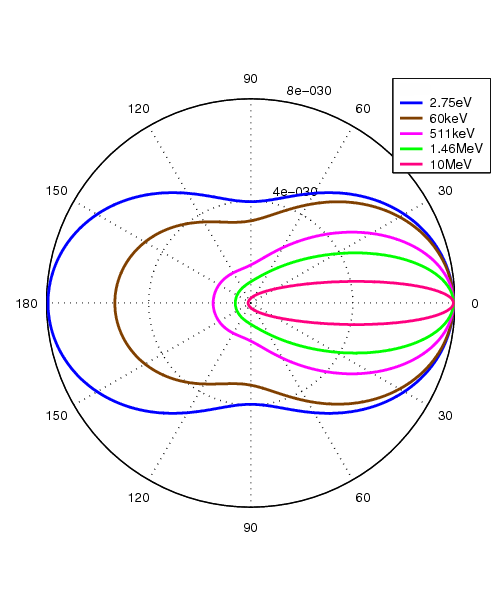
\includegraphics[width=0.5\linewidth]{Klein-Nishina_distribution.png}
  \end{center}
  % Add a caption to describe the figure
  \caption{The differential scattering cross-section 
           $(\frac{d\sigma}{d\Omega})$ predicted by the Klein-Nishina formula
           for photons of various energy}
  % add a label to the figure so you can reference it in the text.
  \label{fig:kn_plot}
\end{figure}

Finally, we want to give Klein and Nishina credit for their work.
We do this by citing the paper where they originally presented their idea.
Fortunately, \LaTeX makes tracking citations $1\times10^{6}$ times easier than
doing it manually.
We can get \LaTeX-formatted citations directly from google scholar (or any
number of other archival programs).
Open a google scholar prompt, and type ``Oscar Klein Yoshio Nishina" in the 
search bar. 
You should get exactly one hit, a nature article from 1928.
Now click the `cite' button under the link, and in the little window that pops
up, click on BibTeX (the name of \LaTeX's citation handler).
This will take you to a page that has the citation perfectly formatted for our
purposes - no manual manipulation required.
Simply copy that data into your references file. In this case, I already did
that in the file I called ``references.bib''.
We can now refer to the paper using the \emph{cite} command and the keyword in
the .bib file that describes the entry, in this case klein1928scattering.
%NOTE: it is common practice, though not required, that these keys follow the
%format <first author's last name><year published><first word of title>.

For more information on the Klein-Nishina formula, please see the original work
in \cite{klein1928scattering}.

\section{Conclusions}

% This is where we actually include the bibliography. It's very easy to do,
% simply choose a style, then include the name of the .bib file that you made
% (without the .bib extension)
\bibliographystyle{plain}
\bibliography{references}

\end{document}
